\section{Conceptos Matematicos}

This Book Template is written in XeLaTeX but you can also change the tamplate to run in PDFLaTeX and whatever you want.\\


\lipsum[1]

\begin{theorem}
    Here goes a theorem.
    \lipsum[1]
\end{theorem}

\begin{proof}
        Here goes the proof

    \lipsum[2]
\end{proof}


\begin{corollary}
    Here goes a collorary
\end{corollary}

\begin{problema}
    Here goes an example
\end{problema}

\begin{note}
    Here goes a note 

    \lipsum[2]
\end{note}


\begin{lemma}
    Here goes a lemma
\end{lemma}

\begin{prop}
    Here goes a proposition
\end{prop}


\begin{definition}
    Here goes a definition 

    \lipsum[2]
\end{definition}

\lipsum[1-2]

\begin{tikznt}
\centering
This box is for  tikz pictures\\\vspace{0.3cm}

\tikzset{every picture/.style={line width=0.75pt}} %set default line width to 0.75pt        

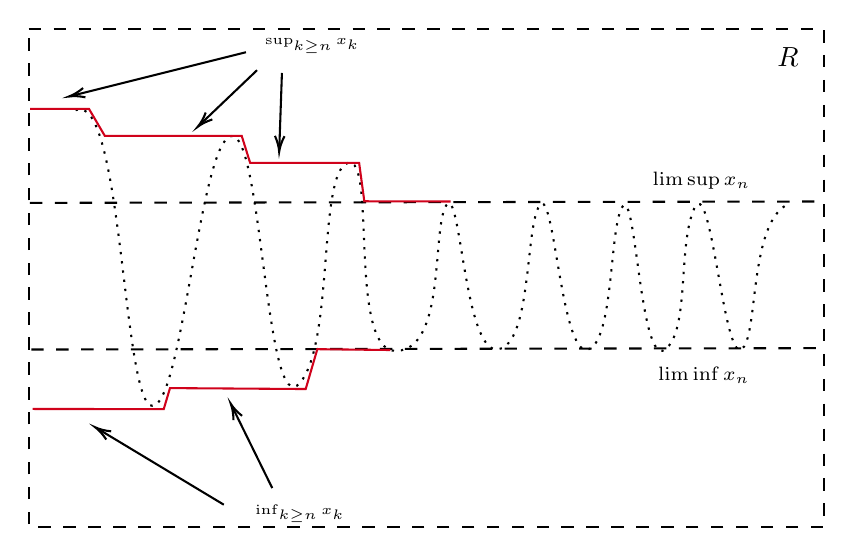
\begin{tikzpicture}[x=0.75pt,y=0.75pt,yscale=-1,xscale=1]
%uncomment if require: \path (0,472); %set diagram left start at 0, and has height of 472

%Curve Lines [id:da44573902991754766] 
\draw  [dash pattern={on 0.84pt off 2.51pt}]  (141.52,165.81) .. controls (164.19,155.81) and (164.19,308.48) .. (178.57,308.29) .. controls (192.95,308.1) and (201.52,180.48) .. (216.57,178.29) .. controls (231.62,176.1) and (232.95,316.76) .. (249.57,297.29) .. controls (266.19,277.81) and (258.19,196.48) .. (272.57,191.29) .. controls (286.95,186.1) and (272.29,282.77) .. (296.19,281.81) .. controls (320.09,280.85) and (313.07,223.21) .. (320.07,211.71) .. controls (327.07,200.21) and (328.62,283.28) .. (345,281) .. controls (361.38,278.72) and (358.07,222.21) .. (365.07,211.71) .. controls (372.07,201.21) and (375.37,284.12) .. (388.19,281.14) .. controls (401.01,278.16) and (398.57,221.71) .. (405.07,212.21) .. controls (411.57,202.71) and (413.52,290.14) .. (425.52,281.14) .. controls (437.52,272.14) and (431.57,231.21) .. (439.57,213.21) .. controls (447.57,195.21) and (453.65,285.77) .. (462.19,281.14) .. controls (470.73,276.52) and (465.52,219.81) .. (485,211) ;
%Straight Lines [id:da2292557377025013] 
\draw  [dash pattern={on 4.5pt off 4.5pt}]  (120.19,281.14) -- (498.86,280.48) ;
%Straight Lines [id:da021754386863272357] 
\draw  [dash pattern={on 4.5pt off 4.5pt}]  (119.52,210.48) -- (500.19,209.81) ;
%Straight Lines [id:da9184013042125718] 
\draw [color={rgb, 255:red, 208; green, 2; blue, 27 }  ,draw opacity=1 ]   (119.57,165.21) -- (148,165.21) -- (155.6,178.17) -- (221.57,178.21) -- (225.64,191.21) -- (278.14,191.21) -- (280.64,209.71) -- (322.19,209.81) ;
%Straight Lines [id:da2894532143841366] 
\draw [color={rgb, 255:red, 208; green, 2; blue, 27 }  ,draw opacity=1 ]   (120.8,309.77) -- (184,309.85) -- (187.02,299.72) -- (252.4,300.17) -- (258,280.97) -- (293.2,281.37) ;
%Straight Lines [id:da09981137612794089] 
\draw    (228.95,146.57) -- (201.73,172.52) ;
\draw [shift={(200.29,173.9)}, rotate = 316.36] [color={rgb, 255:red, 0; green, 0; blue, 0 }  ][line width=0.75]    (7.65,-2.3) .. controls (4.86,-0.97) and (2.31,-0.21) .. (0,0) .. controls (2.31,0.21) and (4.86,0.98) .. (7.65,2.3)   ;
%Straight Lines [id:da7736001528911756] 
\draw    (240.95,147.9) -- (239.69,183.91) ;
\draw [shift={(239.62,185.9)}, rotate = 272.01] [color={rgb, 255:red, 0; green, 0; blue, 0 }  ][line width=0.75]    (7.65,-2.3) .. controls (4.86,-0.97) and (2.31,-0.21) .. (0,0) .. controls (2.31,0.21) and (4.86,0.98) .. (7.65,2.3)   ;
%Straight Lines [id:da01875292146375851] 
\draw    (223.62,137.9) -- (140.23,158.75) ;
\draw [shift={(138.29,159.24)}, rotate = 345.96] [color={rgb, 255:red, 0; green, 0; blue, 0 }  ][line width=0.75]    (7.65,-2.3) .. controls (4.86,-0.97) and (2.31,-0.21) .. (0,0) .. controls (2.31,0.21) and (4.86,0.98) .. (7.65,2.3)   ;
%Straight Lines [id:da685154290163863] 
\draw    (212.95,355.9) -- (152.67,319.6) ;
\draw [shift={(150.95,318.57)}, rotate = 31.05] [color={rgb, 255:red, 0; green, 0; blue, 0 }  ][line width=0.75]    (7.65,-2.3) .. controls (4.86,-0.97) and (2.31,-0.21) .. (0,0) .. controls (2.31,0.21) and (4.86,0.98) .. (7.65,2.3)   ;
%Straight Lines [id:da47753478631845336] 
\draw    (236.29,347.9) -- (217.17,309.03) ;
\draw [shift={(216.29,307.24)}, rotate = 63.81] [color={rgb, 255:red, 0; green, 0; blue, 0 }  ][line width=0.75]    (7.65,-2.3) .. controls (4.86,-0.97) and (2.31,-0.21) .. (0,0) .. controls (2.31,0.21) and (4.86,0.98) .. (7.65,2.3)   ;
%Shape: Rectangle [id:dp6544720458561455] 
\draw  [dash pattern={on 4.5pt off 4.5pt}] (118.95,126.57) -- (502.29,126.57) -- (502.29,366.57) -- (118.95,366.57) -- cycle ;

% Text Node
\draw (418,194.3) node [anchor=north west][inner sep=0.75pt]  [font=\scriptsize]  {$\limsup x_{n}$};
% Text Node
\draw (420.67,288.3) node [anchor=north west][inner sep=0.75pt]  [font=\scriptsize]  {$\liminf x_{n}$};
% Text Node
\draw (231.33,129.97) node [anchor=north west][inner sep=0.75pt]  [font=\tiny]  {$\sup _{k\geq n} x_{k}$};
% Text Node
\draw (226.67,354.64) node [anchor=north west][inner sep=0.75pt]  [font=\tiny]  {$\inf_{k\geq n} x_{k}$};
% Text Node
\draw (478.14,134.26) node [anchor=north west][inner sep=0.75pt]    {$\mathbb{R}$};


\end{tikzpicture}
\end{tikznt}



\subsection{Examples 2}

\lipsum[1-4]
